\documentclass[../main.tex]{subfiles}
\begin{document}

本节中,考虑给定随机向量 $(X_1,\cdots,X_n)$ 和可测函数 $g$,如何求 $Y=g(X_1,\cdots,X_n)$ 的分布。

首先介绍“直接法”。

\begin{example}
    $X_i\sim B(n_i,p)(i=1,2)$ 独立,$Y=X_1+X_2$,则 $\forall k\in\{0,1,\cdots,n_1+n_2\}$,
    \begin{equation*}
        \begin{aligned}
              & P(Y=k)                                                                                               \\
            = & P(X_1+X_2=k)                                                                                         \\
            = & \sum_{k_1=0}^kP(X_1=k_1,X_2=k-k_1)                                                                   \\
            = & \sum_{k_1=0}^kP(X_1=k_1)P(X_2=k-k_1)                                                                 \\
            = & \sum_{k_1=0}^k\tbinom{n_1}{k_1}p^{k_1}(1-p)^{n_1-k_1}\tbinom{n_2}{k-k_1}p^{k-k_1}(1-p)^{n_2-(k-k_1)} \\
            = & \left(\sum_{k_1=0}^k\tbinom{n_1}{k_1}\tbinom{n_2}{k-k_1}\right)p^k(1-p)^{n_1+n_2-k}                  \\
            = & \tbinom{n_1+n_2}{k}p^k(1-p)^{n_1+n_2-k}
        \end{aligned}
    \end{equation*}
    因此 $Y\sim B(n_1+n_2,p)$。
\end{example}

\begin{example}
    随机向量 $(X_1,X_2)$ 有联合 PDF $f(x_1,x_2)$,且 $X_1>0$,考虑 $Y=X_2/X_1$,有 $\forall y\in\mathbb R,P(Y\leq y)=P(\frac{X_2}{X_1}\leq y)=P(X_2\leq X_1y)=\int_Df(x_1,x_2)\mathrm dx_1\mathrm dx_2=\int_0^{+\infty}\int_{-\infty}^{yx_1}f(x_1,x_2)\mathrm dx_2\mathrm dx_1$,作 $x_2=x_1t$ 换元得 $P(Y\leq y)=\int_0^{+\infty}\int_{-\infty}^yf(x_1,x_1t)x_1\mathrm dt\mathrm dx_1$,故 $Y$ 的 PDF 为 $l(y)=\int_0^{+\infty}x_1f(x_1,yx_1)\mathrm dx_1$。

    \begin{figure}[!h]
        \centering
        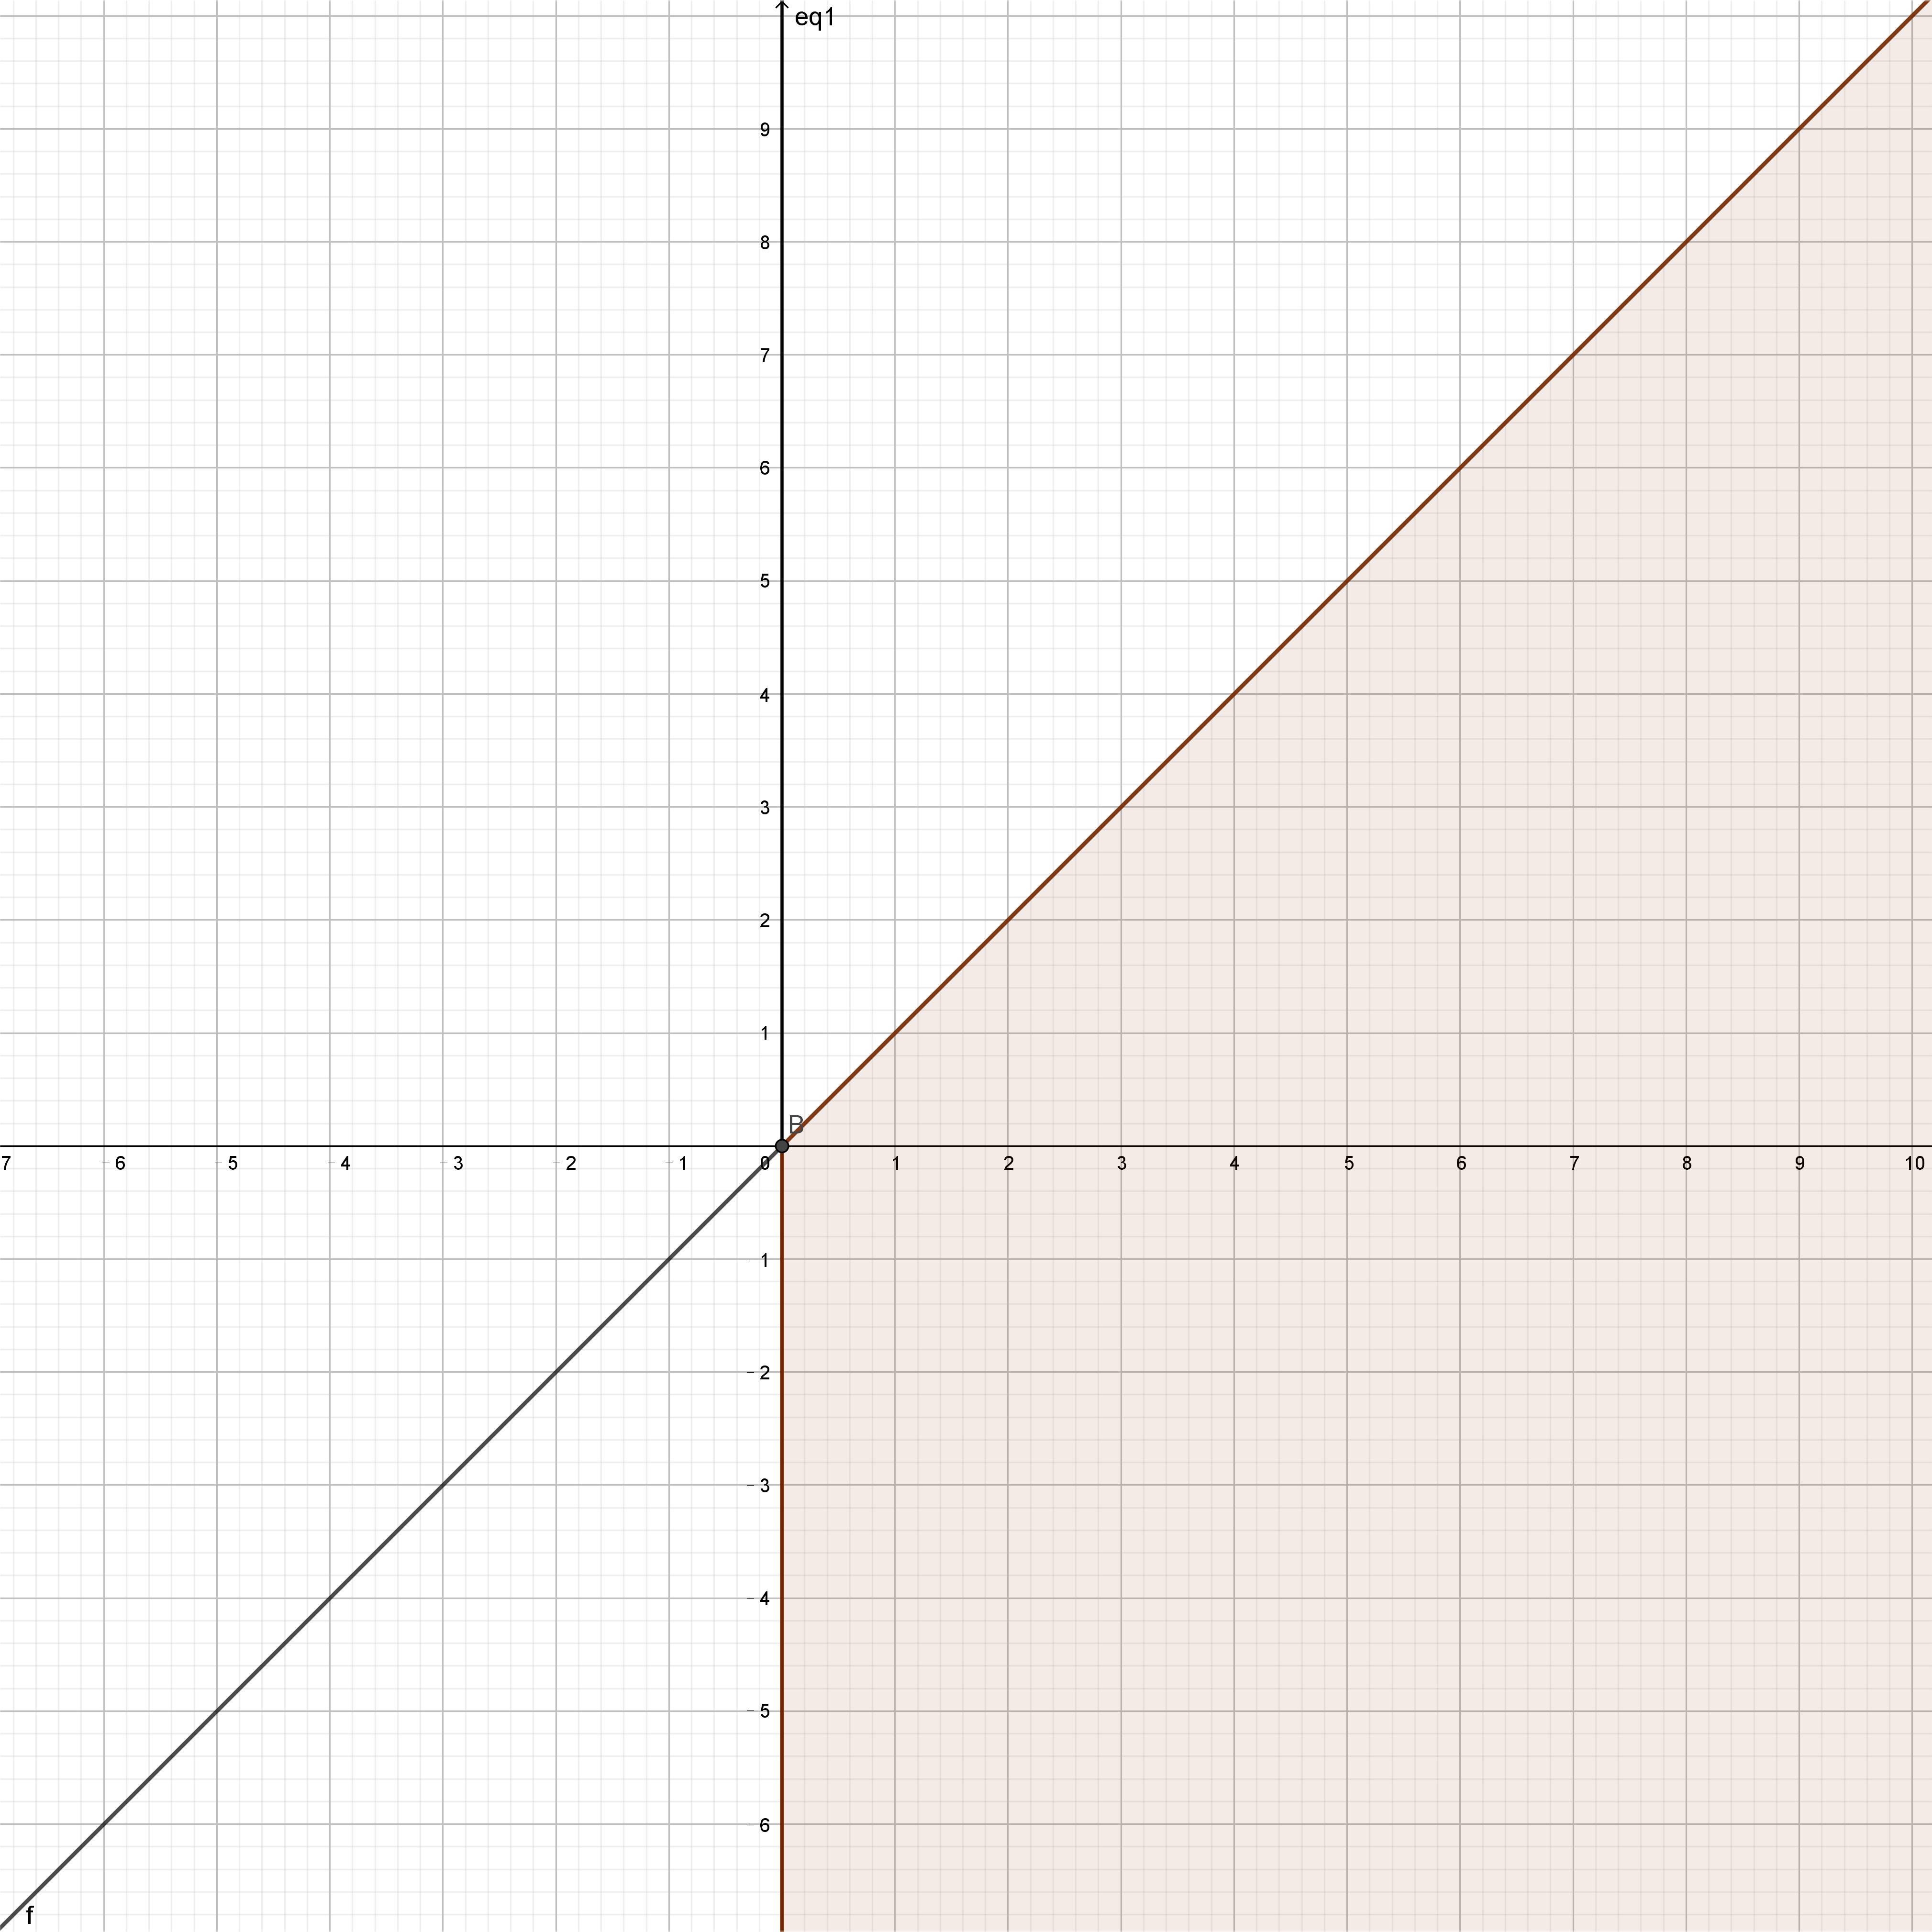
\includegraphics[scale=0.03]{figures/D_area.png}
        \caption{区域 $D$ 的范围,其中边界线的斜率为 $y$}
        \label{fig:3.7.1}
    \end{figure}

\end{example}

接下来介绍“密度函数变换法”。

设随机向量 $(X_1,X_2)$ 有联合 PDF $f(x_1,x_2)$,且有可逆可微的映射关系 $
    \left\{\begin{aligned}
        Y_1 & =g_1(X_1,X_2) \\
        Y_2 & =g_2(X_1,X_2)
    \end{aligned}\right.
$,据此解出逆映射 $
    \left\{\begin{aligned}
        X_1 & =h_1(Y_1,Y_2) \\
        X_2 & =h_2(Y_1,Y_2)
    \end{aligned}\right.
$,则对于任意可测集 $A$,若 $(h_1,h_2)$ 将 $A$ 映射到集合 $B$,则由可逆性可知 $B$ 在 $(g_1,g_2)$ 的映射下的值域为 $A$。因此 $P((Y_1,Y_2)\in A)=P((X_1,X_2)\in B)=\int_Bf(x_1,x_2)\mathrm dx_1\mathrm dx_2=\int_Af(h_1(y_1,y_2),h_2(y_1,y_2))|J|\mathrm dy_1\mathrm dy_2$,其中 $J$ 为 Jacobi 行列式 $
    \det \left[\begin{matrix}
            \frac{\partial h_1}{\partial y_1} & \frac{\partial h_1}{\partial y_2} \\
            \frac{\partial h_2}{\partial y_1} & \frac{\partial h_2}{\partial y_2} \\
        \end{matrix}\right]
$,因此 $(Y_1,Y_2)$ 的联合 PDF 为 $l(y_1,y_2)=f(h_1(y_1,y_2),h_2(y_1,y_2))|J|$。

\begin{example}
    随机向量 $(X_1,X_2)$ 有联合 PDF $f(x_1,x_2)$,为求 $Y=X_1+X_2$ 的 PDF,引入 $Z=X_1$,则 $
        \left\{\begin{aligned}
            X_1 & =Z   \\
            X_2 & =Y-Z
        \end{aligned}\right.
    $,Jacobi 行列式为 $
        \det \left[\begin{matrix}
                0 & 1  \\
                1 & -1
            \end{matrix}\right]=-1
    $
    ,故 $(Y,Z)$ 的联合 PDF 为 $f(z,y-z)|-1|=f(z,y-z)$,$Y$ 的边际 PDF 为 $l_Y(y)=\int_{-\infty}^{+\infty}f(z,y-z)\mathrm dz$。
\end{example}

上例中,若 $X_1,X_2$ 相互独立,则 $f(x_1,x_2)=f_1(x_1)f_2(x_2)\Rightarrow l_Y(y)=\int_{-\infty}^{+\infty}f_1(z)f_2(y-z)\mathrm dz$,这称之为 $f_1$ 和 $f_2$ 的\emph{卷积},记作 $f_1\ast f_2$。

特别地,若 $(X_1,X_2)\sim N(\mu_1,\mu_2,\sigma_1^2,\sigma_2^2,\rho)$,则 $X_1+X_2\sim N(\mu_1+\mu_2,\sigma_1^2+\sigma_2^2+2\rho\sigma_1\sigma_2)$。

利用上述随机向量的函数的 PDF 求解方法,可以得到所谓卡方分布($\chi^2$-分布)、$t$-分布和 $F$-分布的 PDF。这些分布的表达式较为复杂,在此不一一罗列。感兴趣的同学可以查阅资料,简单了解一下它们与标准正态分布的联系。

\end{document}
